Frequencies or counts of specific observations build the foundation of the visualizations used. More specific frequency distributions are used, as they allow to organize the available model validation results in a meaningful way, which connects the knowledge gained through validation with the structure of the model to be explained. Basically, a frequency distribution table is used to show the different measurement categories and the number of observations per category.

\begin{Def}{Frequency Distribution Table \cite{manikandan2011frequency}}{frequency_distribution_tables}
A frequency distribution table $F_{C_1,C_2,...,C_n} \in \mathbb{N}^{|C_1| \times |C_2| \times ... \times |C_n|}$ is an n-dimensional matrix of natural numbers, where $C_1, C_2, ... , C_n$ are sets of measurement categories. 
\end{Def}

Therefore, independent of the model, the easiest frequency distribution table would have the validation results as the single group of measurement categories and, hence, can be visualized by a pie chart. This kind of visualization can be used as a very raw summary of the validation results.

\begin{Bsp}{A First Visualization for the Example Constraint}{samples_for_indices_plot}
    First, it should be noted that the example constraint is a prediction constraint and, therefore, it is assumed that the underlying semantic context of the samples in the knowledge graph is correct. 
    The validation results are already given in example \ref{Bsp:evaluating_example_constraint}, from which a frequency distribution table is build, having the validation results as categories for both kinds of semantics (see Figure \ref{fig:samples_for_indices_table_2valued} and \ref{fig:samples_for_indices_table_3valued}). This kind of one dimensional data is easily visualized by a pie chart as shown in Figure \ref{fig:samples_for_indices_plot_2valued} and \ref{fig:samples_for_indices_plot_3valued}. As a pie chart converts frequencies into fractions, the number $n$ of samples in the dataset are given below the chart. Comparing the two visualizations, the 3-valued one gives more information, as it becomes clear, that there are not many pregnant persons in Germany, which have more than 20 contacts to not vaccinated persons in the dataset. Further, the pie chart shows that the few to which the constraint applies, the model recommends not getting vaccinated, which invalidates the predictions. 
    
    \captionsetup{type=htypei}
    \begin{minipage}[t]{\linewidth}
        \vspace{1ex}
        \centering
        \begin{tabular}{l|cc}
            \toprule
             Groups & invalid & valid\\
             \midrule
             Complete Dataset & 833 & 9166\\
             \bottomrule
        \end{tabular}    
        \captionof{figure}{Frequency distribution table $F_{\{0,1\}}$ using the 2-valued logic for the motivating example constraint}
        \label{fig:samples_for_indices_table_2valued}
    \end{minipage}
    
    \captionsetup{type=htypei}
    \begin{minipage}[t]{\linewidth}
        \vspace{1ex}
        \centering
        \begin{tabular}{l|ccc}
            \toprule
             Groups & not applicable & invalid & valid \\
             \midrule
             Complete Dataset & 9166 & 833 & 0 \\
             \bottomrule
        \end{tabular}  
        \captionof{figure}{Frequency distribution table $F_{\{-1,0,1\}}$ using the 3-valued logic for the motivating example constraint}
        \label{fig:samples_for_indices_table_3valued}
    \end{minipage}.

    \begin{minipage}[t]{\linewidth}
    \vspace{1ex}
    \centering
        \captionsetup{type=htypei}
        \begin{minipage}[t]{0.4\linewidth}
            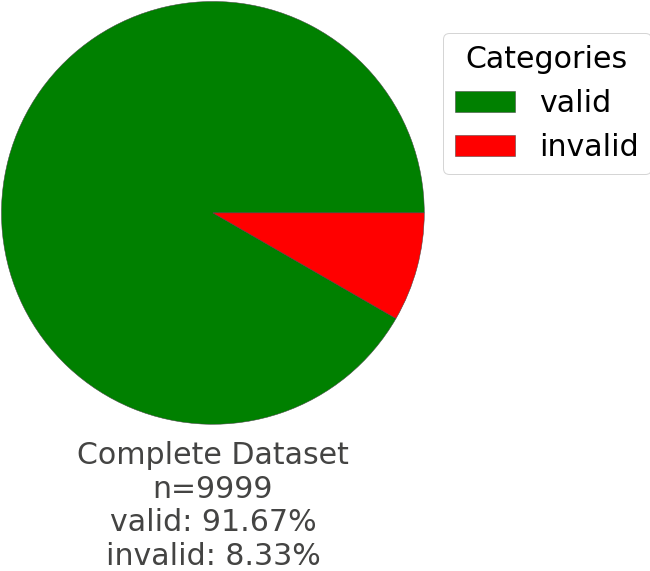
\includegraphics[scale=.25]{images/visualizations/sample_for_all_indices_2valuedlogic.png}    
            \captionof{figure}{Pie Chart of the frequency distribution table in Figure \ref{fig:samples_for_indices_table_2valued}}
            \label{fig:samples_for_indices_plot_2valued}
        \end{minipage}
        \hspace{1ex}
        \captionsetup{type=htypei}
        \begin{minipage}[t]{0.4\linewidth}
            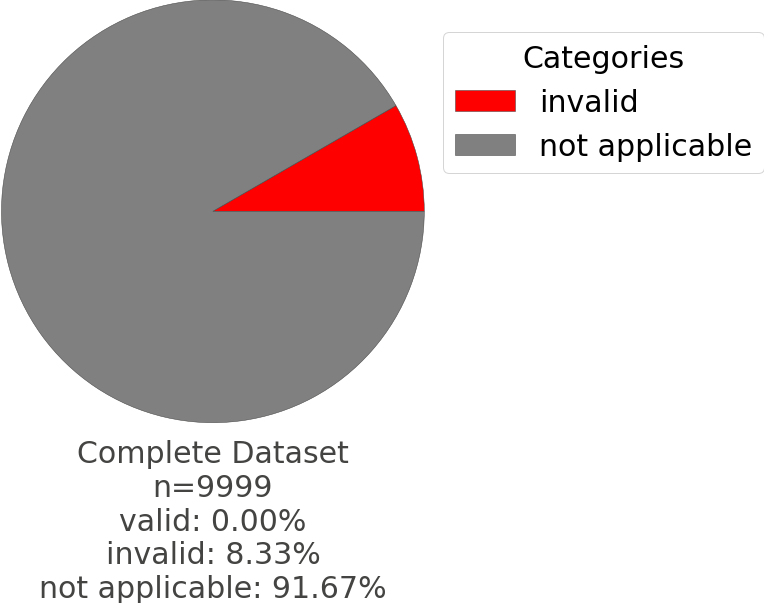
\includegraphics[scale=.25]{images/visualizations/sample_for_all_indices_3valuedlogic.png}        
            \captionof{figure}{Pie Chart of the frequency distribution table in Figure \ref{fig:samples_for_indices_table_3valued}}
            \label{fig:samples_for_indices_plot_3valued}
        \end{minipage}
    \end{minipage}
\end{Bsp}

In a next step, this kind of frequency distributions are extended by splitting the dataset into different groups. Depending on the machine learning task, one might create a group for each class (classification) or have a range of target values for each group (regression). In both cases the grouping can be made depending on the prediction of the model or based on the ground truth target value in the dataset. As the data is now two-dimensional, a histogram can be used for visualization.

\begin{Bsp}{Group by Target for more Meaningful Visualisations}{class_per_constraint_samples_plot}
    Here the 3-valued logic is used and the frequency distribution from example \ref{Bsp:samples_for_indices_plot} is extended, such that each ground truth class builds a separate group. As the validation results from \ref{Bsp:evaluating_example_constraint} are used, the model, which is validated, is the decision tree in Figure \ref{motivating_example_decision_tree} and the predicted class equals the ground truth class in that case for all samples in the dataset. Besides this fact, the histogram shows that the invalidated predictions were made on the basis of falsely labeled data. The corresponding histogram is shown in Figure \ref{fig:class_per_constraint_samples_plot}.
    
    \captionsetup{type=htypei} 
    \begin{minipage}[t]{\linewidth}
        \vspace{1ex}
        \centering
        \begin{tabular}{l|ccc}
            \toprule
             Groups & valid & invalid & not applicable \\
             \midrule
             vaccinated & 0 & 0 & 5000 \\
             not vaccinated & 0 & 833 & 4166 \\
             \bottomrule
        \end{tabular}    
        \captionof{figure}{Frequency distribution table $F_{\{\textrm{vaccinated},\textrm{not vaccinated}\},\{-1,0,1\}}$ for the motivating example constraint using a grouping by the target class}
        \label{fig:class_per_constraint_samples_table}
    \end{minipage}
        \captionsetup{type=htypei}
        \begin{minipage}[t]{\linewidth}
            \vspace{1ex}
            \centering
            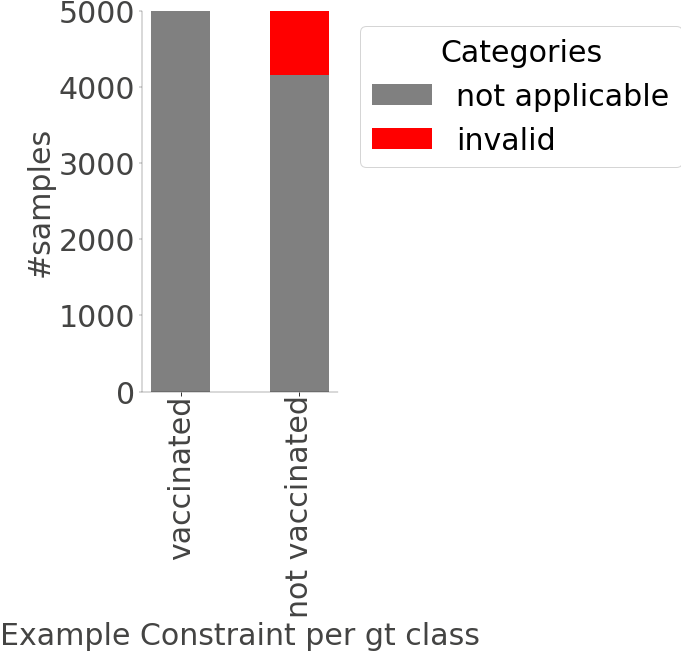
\includegraphics[scale=.25]{images/visualizations/example_constraint_per_gt_class.png}    
            \captionof{figure}{Histogram of the frequency distribution table in Figure \ref{fig:class_per_constraint_samples_table}}
            \label{fig:class_per_constraint_samples_plot}
        \end{minipage}
\end{Bsp}

In the last two examples, the complete dataset is used to build the frequency distribution table. But clearly this does not need to be the case. It might be useful to summarize only a fraction of the constraint validation results belonging to specific samples in the dataset. As the table is created dependent on a constraint, which completes the components needed to define the frequency distribution tables used to summarize the validation results.

\begin{Def}{A Function to Create Frequency Distribution Tables to Summarize Model Validation Results given one Constraint}{frequency_distribution_creation_function}
Let $D$ be a dataset, $G$ a set of arbitrary group identifiers, $C$ a constraint, $N$ the number of samples in $D$ and $\mathbf{\Gamma}$ the endless space of grouping function $\Gamma: G \to \mathcal{P}([1,...,N])$, then the function \[\mathcal{F}_{G,C}: \mathcal{P}([1,...,N]) \times \mathbf{\Theta} \times \mathbf{\Gamma} \to \mathbb{N}^{|G| \times |\{-1,0,1\}|}\] maps a subset of the indices $D_{idx}$ of $D$, a model validation result function $\Theta$ and a grouping function $\Gamma$ to a frequency distribution table:
 \[\mathcal{F}_{G,C}(D_{idx},\Theta, \Gamma) \mapsto F_{G,\{-1,0,1\}}^{C,D_{idx}}\]
 where
 \[F_{G,\{-1,0,1\}}^{C,D_{idx}} = \left(\left|f_{g,v}^{C,D_{idx}}\right|\right)_{\substack{g \in G\\ v \in \{-1,0,1\}}}\]
 \[f_{g,v}^{C,D_{idx}} = \{ i | i \in (D_{idx} \cap \Gamma(g)) \land \Theta(C,i) = v\}\]
Clearly $\Theta$, $\Gamma$ and $D_{idx}$ have to refer to the same dataset $D$.
\end{Def}

The definition concludes the creation of frequency distribution tables for one constraint given a dataset (a tuple of samples), the model validation result function and a function used for grouping. The following example shows the application of definition \ref{Def:frequency_distribution_creation_function} using the previous examples.

\begin{Bsp}{Creating Frequency Distribution Tables Formally}{creating_frequency_distribution_tables}
Example \ref{Bsp:samples_for_indices_plot} and example \ref{Bsp:class_per_constraint_samples_plot} both created frequency distribution tables. Both of them use the whole dataset ($D_{full} = [1,...,N])$ as shown in example \ref{Bsp:sample-to-node_mapping_motivating_example}, the model-validation-result $\Theta$ function as shown in example \ref{Bsp:evaluating_example_constraint} and the constraint $C$ defined in example \ref{Bsp:motivating_example_constraint_definition}. 

In example \ref{Bsp:samples_for_indices_plot}, there is only a single group. Therefore, $\Gamma_\textrm{all}$, would be the function mapping all indices of instances in $D$ to the same group called \emph{Complete Dataset}. Therefore, to create the frequency distribution table in Figure \ref{fig:samples_for_indices_table_3valued} the following formula is evaluated.
\[
    \mathcal{F}_{\{\textrm{Complete Dataset}\},C}(D_{full},\Theta, \Gamma_{\textrm{all}})
\]
In the second example, two grouping functions are used such that instances with the same predicted target class or ground truth target class are grouped together. In the first case, it holds

\[\Gamma_{\textrm{predicted class}}(g) \mapsto \{i \mid M_\theta(i) = g\}\]
and in the second case
\[\Gamma_{\textrm{ground truth class}}(g) \mapsto \{i \mid t_i = g\}\]
Therefore, creating the frequency distribution table corresponding to Figure \ref{fig:class_per_constraint_samples_table} is a matter of executing
\[
    \mathcal{F}_{\{\textrm{vaccinated}, \textrm{not vaccinated}\},C}(D_{full},\Theta, \Gamma_{\textrm{predicted class}})
\]
or 
\[
    \mathcal{F}_{\{\textrm{vaccinated}, \textrm{not vaccinated}\},C}(D_{full},\Theta, \Gamma_{\textrm{ground truth class}})
\]
\end{Bsp}

In definition \ref{Def:frequency_distribution_creation_function} the domain of the grouping function $\textrm{dom}(\Gamma)$ is one dimensional, but clearly multiple grouping functions $\Gamma_1,\Gamma_2,...,\Gamma_M$ with domains $G_1,G_2,...,G_M$ can be combined to give a function $\Gamma_{[1,...,M]}: G_1 \times G_2 \times... \times G_M \to \mathcal{P}([1,...,N])$ with

\begin{gather}
    \Gamma_{[1,2,...,M]}(g_1,g_2,...,g_M) \mapsto \bigcap_{i \in [1,...,M]} \Gamma_i(g_i) \label{multiple_grouping_functions_to_one}
\end{gather}

where $(g_1,g_2,...,g_M) \in G_1 \times G_2 \times ... \times G_M$. Setting $G = G_1 \times G_2 \times ... \times G_M$ allows to generalize the definition to multidimensional grouping functions.

